\chapter{EPL and Esper}

\section{What is Esper?}

Esper is an open-source software product for Complex Event Processing (CEP) and
Stream Analytics, developed by EsperTech. It turns a large amount of incoming
event series or streams into actionable insights in real-time. It is a
lightweight, high-performance, and scalable engine that can process millions of
events per second.\\

Esper provides a SQL-like language called EPL (Event Processing Language) to
define queries and patterns over event streams. It also provides a Java API to
integrate with Java applications.\\

\begin{figure}[H]
    \centering
    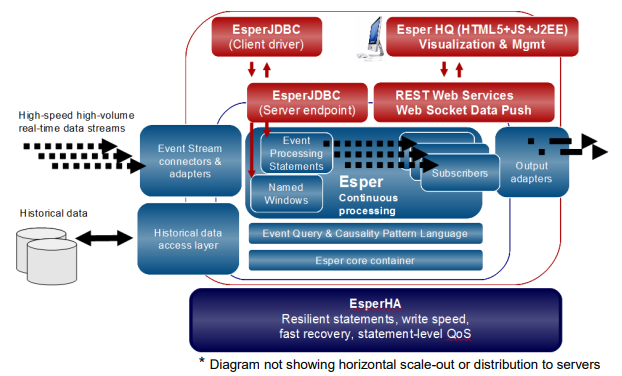
\includegraphics[width=0.6\textwidth]{figures/image_esper.png}
    \caption{Esper Architecture}
    \label{fig:esper}
\end{figure}

\subsection{Esper features}

\begin{itemize}
    \item It is implemented as a Java library, so it can be easily integrated with
    Java applications.

    \item It provides a SQL-like language called EPL to define queries and patterns
    over event streams.

    \item it is designed for performance and scalability, and it can process millions
    of events per second (high throughput and low latency).

    \item It can interact with static/historical data, and it can be used to
    correlate real-time data with historical data.

    \item It has a configurable push and pull communication.
\end{itemize}

\section{EPL in a nutshell}

EPL is a SQL-like language that allows you to define queries and patterns over
event streams. It is used to define the logic that Esper uses to process events.\\

As in the DSMS approach, it offers stream-to-relation operators, e.g., windowing, 
relation-to-relation operators, like joins, proections, selections, and aggregation;
and relation-to-stream operators to produce output. As in the CEP approach, it offers 
a comprehensive set of operators to define and detect patterns in event streams.\\

EPL is similar to SQL, as seen in some of its syntax (e.g., \texttt{SELECT}, \texttt{FROM},
\texttt{WHERE}, \texttt{GROUP BY}, etc.). However, it is based on event streams 
and views, rather than tables. Here, views define the data that is available for
queries, they can represent windows over streams, and they can also sort events, derive
statistics from event attributes, group events, etc.

\section{EPL syntax: fire alarms example}

To learn more about its syntax, let us consider the following example. Suppose we have
a set of fire alarms that send events when they detect smoke. We want to detect when a
fire is happening by correlating the events from the fire alarms. Specifically, to 
detect a fire, we need to receive a smoke event followed by a temperature $> 50$ event,
within 2 minutes, at the same sensor.\\

In this section, we will learn how to:

\begin{itemize}
    \item Define event types as schemas
    \item Create simple queries
    \item Define different types of windows
    \item Personalize the output stream
    \item Recognize complex patterns of events
\end{itemize}

\subsection{Creating a schema}

In EPL, we can define schemas to define the structure of the events that we are
going to process. They are useful to register and recognize specific event types
when creating queries, especially the most complex ones.\\

To define a schema, we mainly use the \texttt{CREATE SCHEMA} statement, although
we can also use the runtime configuration API \texttt{addEventType} method.
We use the following syntax:\\

\begin{lstlisting}[language=SQL]
create schema --keyword to create a schema
schema_name [as...] --name of schema (you can add an alias)
(
    field_name data_type [,...] --field name and data type
    [inherits inherited_schema_name] --it can inherit from another schema
);
\end{lstlisting}

In our example, we need to describe 3 types of events: smoke events, temperature
events, and fire events. For that, we can define the following schemas:\\

\begin{lstlisting}[language=SQL]
create schema SmokeSensorEvent (
    sensor string,
    smoke boolean,
);

create schema TemperatureSensorEvent (
    sensor string,
    temperature double,
);

create schema FireEvent (
    sensor string,
    smoke boolean,
    temperature double,
);
\end{lstlisting}

\subsection{Creating a simple query}

In EPL, we can define queries in the same way we do in SQL. We can use the
\texttt{SELECT} statement to select fields, the \texttt{FROM} statement to select
from a stream, the \texttt{WHERE} statement to filter the data, and so on. Let's
see the following example:\\

\begin{lstlisting}[language=SQL]
@Name('Query_0')
select *
from TemperatureSensorEvent
where temperature > 50;
\end{lstlisting}

In this query, we are selecting all fields from the \texttt{TemperatureSensorEvent}
stream where the temperature is greater than 50. However, in this case, the query is 
getting executed every time a new event arrives, so it is not efficient. We can consider
using an event-based system style, like this:\\

\begin{lstlisting}[language=SQL]
@Name('Query_0_BIS')
select *
from TemperatureSensorEvent(temperature > 50);
\end{lstlisting}

In this way, the events are filtered before being processed by the query, which is
a little more efficient. \\

We could also want to obtain the results of each sensor separately. For that, we
can use the \texttt{GROUP BY} statement, as follows:\\

\begin{lstlisting}[language=SQL]
@Name('Query_1')
select sensor, avg(temperature)
from TemperatureSensorEvent
group by sensor;
\end{lstlisting}

In this query, we are selecting the sensor and the average temperature from the
corresponding stream, grouping by sensor. This way, we can obtain the average
temperature of each sensor, observed in the whole stream.

\subsection{Defining windows}

In EPL, we can define windows to group events in time or in the number of events.
There are 2 main types of windows, regarding the chosen time model: logical windows, 
that are based on absolute time, and physical windows, that are based on the 
ocurrence of events.\\

From each type, we can define 3 subtypes: tumbling windows, sliding windows, and
hopping windows. We will see how to define each one of them.

\subsubsection{Tumbling windows}

Tumbling windows are the simplest type of windows. They divide the stream into
fixed-size, non-overlapping windows. This size may be measured in absolute time
(logical tumbling windows) or in the number of events (physical tumbling windows).\\

To use a logical tumbling window, we use the following syntax:\\

\begin{lstlisting}[language=SQL]
@Name('Query_2')
select sensor, avg(temperature)
from TemperatureSensorEvent.win:time_batch(4 seconds)
group by sensor;
\end{lstlisting}

In this query, we are selecting the sensor and the average temperature from the
corresponding stream, grouping by sensor, and using a logical tumbling window of
4 seconds. This way, we can obtain the average temperature of each sensor, observed
in the last 4 seconds, every 4 seconds.\\

We can also use physical tumbling windows, as follows:\\

\begin{lstlisting}[language=SQL]
@Name('Query_3')
select sensor, avg(temperature)
from TemperatureSensorEvent.win:length_batch(4)
group by sensor;
\end{lstlisting}

In this way, we can obtain the average temperature of each sensor, observed in the 
last 4 events, every 4 events.\\

\subsubsection{Sliding windows}

Sliding windows are a more complex type of windows. They are defined by
every event that arrives in the stream, and they can overlap. The slide size
is determined either by the time (logical) or by a number of events (physical).\\

To use a sliding window, we use the following syntax:\\

\begin{lstlisting}[language=SQL]
@Name('Query_4')
select sensor, avg(temperature)
from TemperatureSensorEvent.win:time(4 seconds)
group by sensor;
\end{lstlisting}

In this query, we obtain the average temperature of each sensor, observed
in the last 4 seconds, every time an event arrives.\\

If we want to use a physical sliding window, we can use the following syntax:\\

\begin{lstlisting}[language=SQL]
@Name('Query_5')
select sensor, avg(temperature)
from TemperatureSensorEvent.win:length(4)
group by sensor;
\end{lstlisting}

In this query, we obtain the average temperature of each sensor, observed
in the last 4 events, every time an event arrives.\\

\subsubsection{Hopping windows}

Hopping windows are a combination of tumbling and sliding windows. They are
defined by a fixed-size window that slides by a fixed-size increment. This type
of windows tend to overlap. The window size is determined either by the time 
(logical) or by a number of events (physical).\\

To use a hopping window, we use the following syntax:\\

\begin{lstlisting}[language=SQL]
@Name('Query_6')
select sensor, avg(temperature)
from TemperatureSensorEvent.win:time(4 seconds)
group by sensor;
output snapshot every 2 seconds;
\end{lstlisting}

Notice that to use a hopping window, we need to specify the hopping length by
modifying the output stream. In this query, we obtain the average temperature of
each sensor, observed in the last 4 seconds, every 2 seconds.\\

Now, let's deepen our knowlegde about how to personalize the output stream.

\subsection{Output stream}

In EPL, we can declare output policies to define how the output stream is going
to be generated. We use the \texttt{OUTPUT} statement, followed by the desired
policy. Also, with the \texttt{EVERY} keyword, we can specify the frequency of 
the output.\\

There are 4 main types of output policies: snapshot, all, first, and last.
Let's see how to use each one of them:

\begin{itemize}
    \item Snapshot: it generates a snapshot of the current state of the window.
    \item All: it generates all the events in the window that matches the query.
    \item First: it generates the first event in the window that matches the query.
    \item Last: it generates the last event in the window that matches the query.
\end{itemize}

Let's see an example of this:\\

\begin{lstlisting}[language=SQL]
@Name('Query_7_SNAP')
select sensor, avg(temperature)
from TemperatureSensorEvent.win:time(4 seconds)
group by sensor;
output snapshot every 2 seconds;

@Name('Query_7_ALL')
select sensor, avg(temperature)
from TemperatureSensorEvent.win:time(4 seconds)
group by sensor;
output all every 2 seconds;

@Name('Query_7_FIRST')
select sensor, avg(temperature)
from TemperatureSensorEvent.win:time(4 seconds)
group by sensor;
output first every 2 seconds;

@Name('Query_7_LAST')
select sensor, avg(temperature)
from TemperatureSensorEvent.win:time(4 seconds)
group by sensor;
output last every 2 seconds;
\end{lstlisting}

In this example, we are obtaining the average temperature of each sensor, observed
in the last 4 seconds, every 2 seconds, using the snapshot, all, first, and last
output policies.\\

The main difference between \texttt{SNAPSHOT} and \texttt{ALL} is that the former
generates a snapshot of the current state of the window, while the latter generates
all the events in the window that matches the query, no matter if they are a null 
event.

\subsection{Complex event patterns}

In EPL, we can define complex event patterns to detect specific sequences of events
in the stream. We use the \texttt{PATTERN} statement, followed by the desired pattern.
Let's see an example of this:\\

\begin{lstlisting}[language=SQL]
@Name('Query_8')
select *
from pattern [
    a=SmokeSensorEvent(smoke=true) ->
    b=TemperatureSensorEvent(temperature > 50, sensor = a.sensor)
];
\end{lstlisting}

This query is searching for a smoke event followed by a temperature $> 50$ event.
Note that this query only matches the first occurrence of the pattern. If we want
to match all the occurrences, we should use the \texttt{EVERY} keyword.

\subsubsection{\texttt{EVERY} clause}

The \texttt{EVERY} clause is used to re-start the pattern matching process after
a successful or failed match. It has different approaches:

\begin{itemize}
    \item \texttt{EVERY (A -> B)}: it matches the pattern every time the event
    A is followed by the event B. The moment the event B is matched, the
    pattern matching process is re-started, and the event A is expected again.

    \begin{figure}[H]
        \centering
        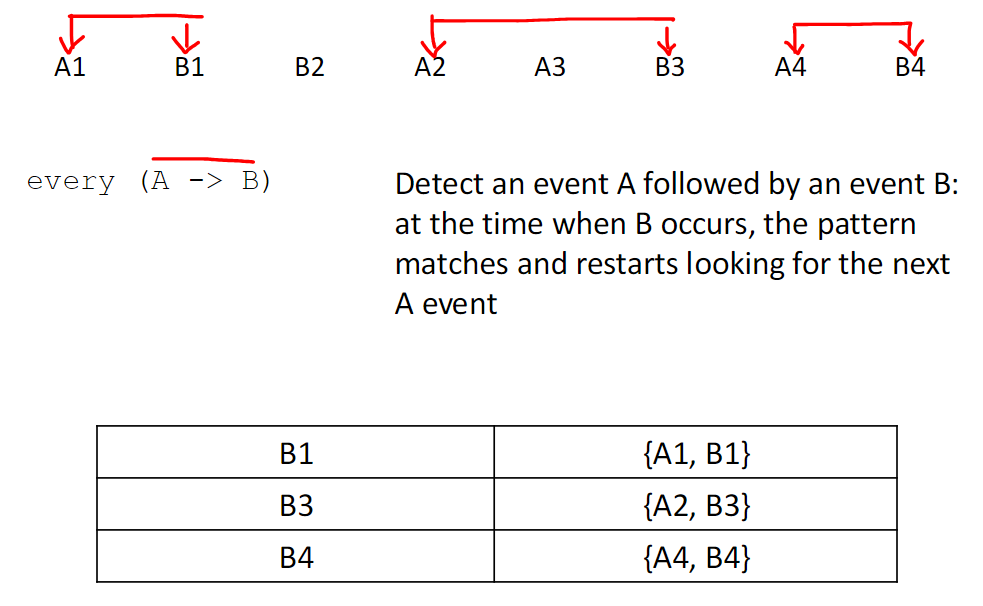
\includegraphics[width=0.5\textwidth]{figures/image_everyAB.png}
        \caption{Pattern matching with \texttt{EVERY (A -> B)}}
        \label{fig:pattern_1}
    \end{figure}

    Let's see an example of this:\\

    \begin{lstlisting}[language=SQL]
@Name('Query_9')
select *
from pattern [
    every (
        a=SmokeSensorEvent(smoke=true) 
        ->
        b=TemperatureSensorEvent(temperature > 50, sensor = a.sensor)
    )
];
    \end{lstlisting}

    \item \texttt{EVERY A -> B}: it matches the pattern every time the event A is
    followed by the event B. In this case, the pattern matching process fires every
    time an event A is matched, and succesfully returns when the event B is matched, 
    so it will return every A followed by B.

    \begin{figure}[H]
        \centering
        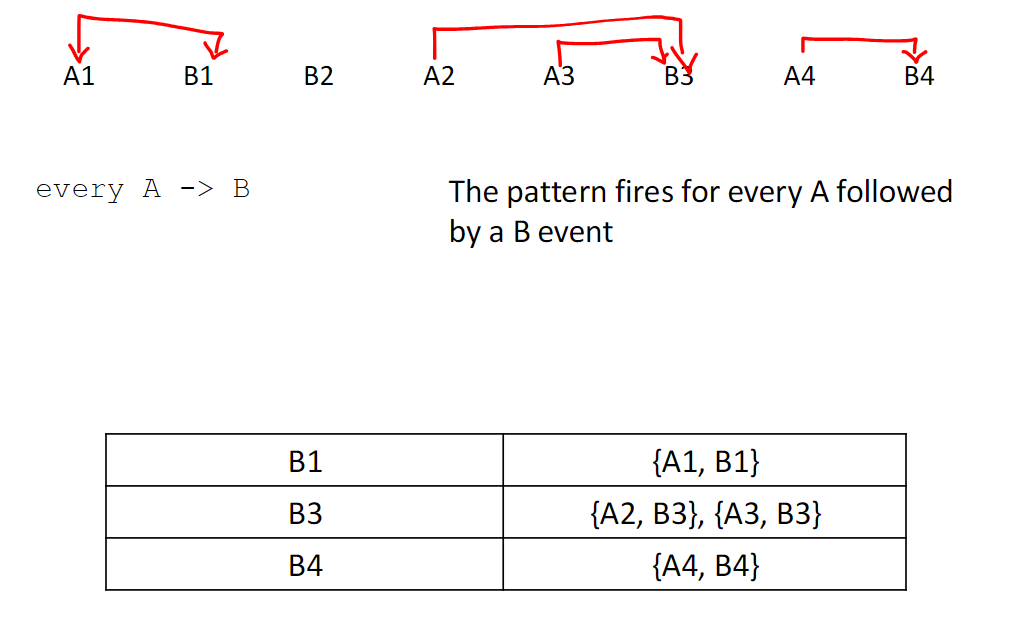
\includegraphics[width=0.5\textwidth]{figures/image_everyA_B.png}
        \caption{Pattern matching with \texttt{EVERY A -> B}}
        \label{fig:pattern_2}
    \end{figure}

    Let's see an example of this:\\

    \begin{lstlisting}[language=SQL]
@Name('Query_10')
select *
from pattern [
    every a=SmokeSensorEvent(smoke=true) 
        ->
        b=TemperatureSensorEvent(temperature > 50, sensor = a.sensor)
];
    \end{lstlisting}

    \item \texttt{A -> EVERY B}: it matches the pattern every time the event A is
    followed by the event B. In this case, once the event A is matched, this pattern
    will be matched every time the event B is encountered, so it will return every B
    following that A.

    \begin{figure}[H]
        \centering
        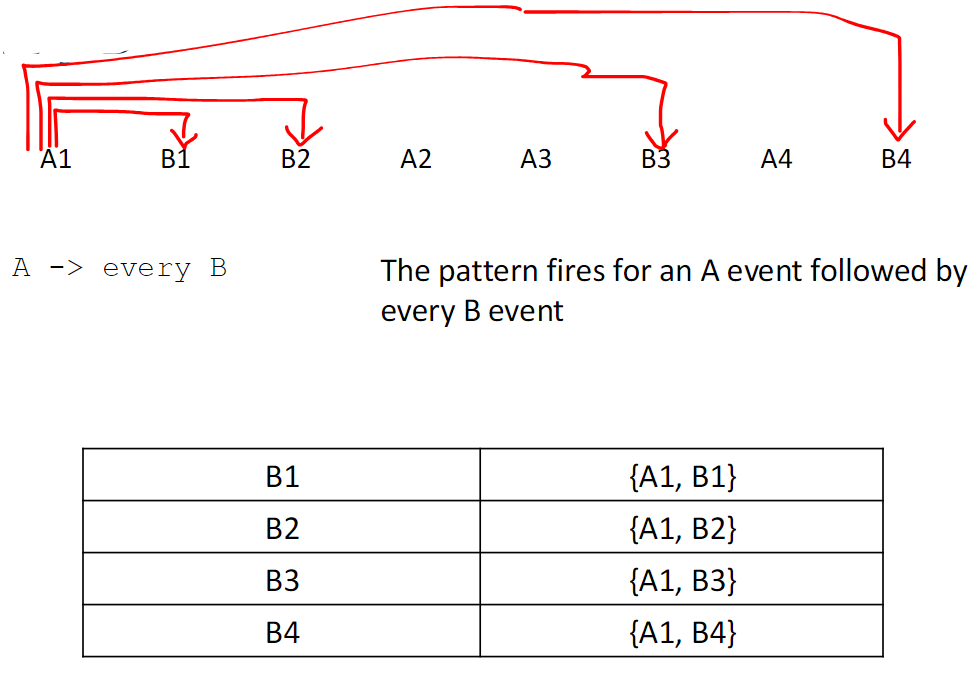
\includegraphics[width=0.5\textwidth]{figures/image_A_everyB.png}
        \caption{Pattern matching with \texttt{A -> EVERY B}}
        \label{fig:pattern_3}
    \end{figure}

    Let's see an example of this:\\

    \begin{lstlisting}[language=SQL]
@Name('Query_11')
select *
from pattern [
    a=SmokeSensorEvent(smoke=true) 
        ->
        every b=TemperatureSensorEvent(temperature > 50, sensor = a.sensor)
];
    \end{lstlisting}

    \item \texttt{EVERY A -> EVERY B}: it matches the pattern every time the event
    A is followed by the event B. In this case, the pattern matching process fires
    every time an event A is matched, and for each A, it will return every B that
    follows that A.

    \begin{figure}[H]
        \centering
        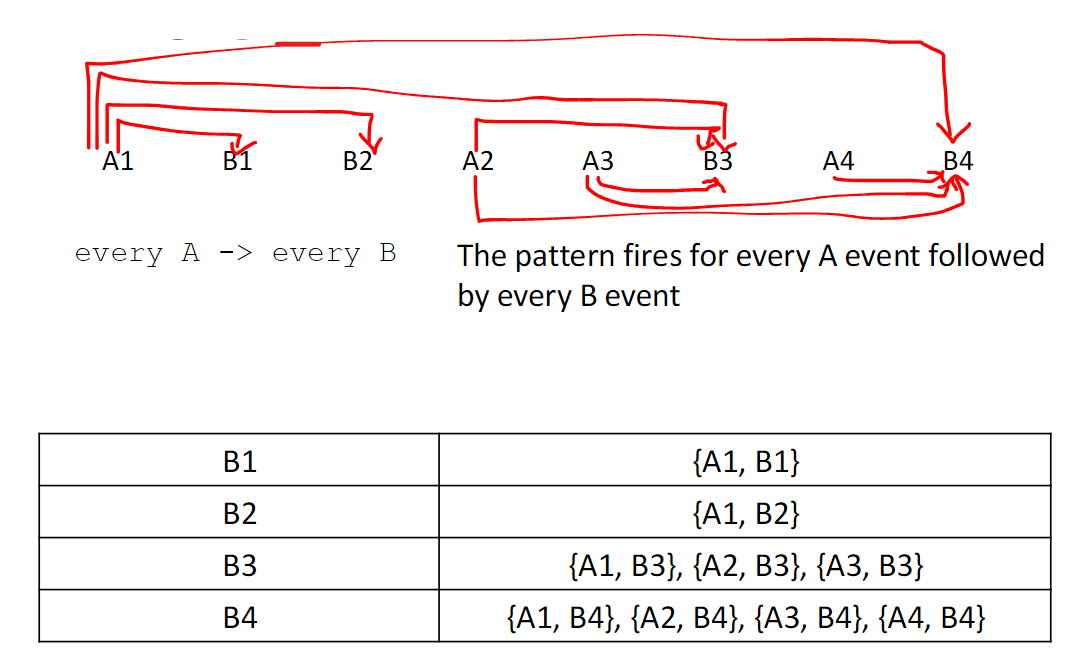
\includegraphics[width=0.5\textwidth]{figures/image_everyA_everyB.png}
        \caption{Pattern matching with \texttt{EVERY A -> EVERY B}}
        \label{fig:pattern_4}
    \end{figure}

    Let's see an example of this:\\

    \begin{lstlisting}[language=SQL]
@Name('Query_12')
select *
from pattern [
    every a=SmokeSensorEvent(smoke=true) 
        ->
        every b=TemperatureSensorEvent(temperature > 50, sensor = a.sensor)
];
    \end{lstlisting}

\end{itemize}

Note that the \texttt{EVERY} clause restarts the pattern matching process multiple times.
This can be very resource-intensive, so it should be used with caution. Also, we don't always
want to match every pattern in the stream, but only in an specific window, or in an specific 
context. For that, we have pattern guards.

\subsubsection{Pattern guards}

Pattern guards are used to restrict the pattern matching process to a specific context.
There are 2 main types of pattern guards: \texttt{TIMER:WITHIN} and \texttt{AND NOT}.
Let's see how to use each one of them:

\begin{itemize}
    \item \texttt{TIMER:WITHIN}: it restricts the pattern matching process to a specific
    time window. It is used to specify a time limit for the pattern matching process.
    Let's see an example of this:\\

    \begin{lstlisting}[language=SQL]
@Name('Query_13')
select *
from pattern [
    a=SmokeSensorEvent(smoke=true) 
        ->
        b=TemperatureSensorEvent(temperature > 50, sensor = a.sensor)
    where timer:within(2 minutes)
];
    \end{lstlisting}

    In this query, we are searching for a smoke event followed by a temperature $> 50$
    event, within 2 minutes. This way, we are restricting the pattern matching process
    to a specific time window.

    \item \texttt{AND NOT}: it restricts the pattern matching process to exclude specific
    events. It is used to specify that an event should not be matched. Let's see an example
    of this:\\

    \begin{lstlisting}[language=SQL]
@Name('Query_14')
select *
from pattern [
    a=SmokeSensorEvent(smoke=true) 
        ->
        b=TemperatureSensorEvent(temperature > 50, sensor = a.sensor)
    and not c=FireEvent(sensor = a.sensor)
];
    \end{lstlisting}

    In this query, we are searching for a smoke event followed by a temperature $> 50$
    event, and excluding the case when a fire event is detected at the same sensor.
    This way, we are restricting the pattern matching process to exclude specific events.

\end{itemize}

\subsubsection{Operators precedence}

For all these operations, we need to consider the operators precedence. The operators
are evaluated in the following order:

\begin{figure}[H]
    \centering
    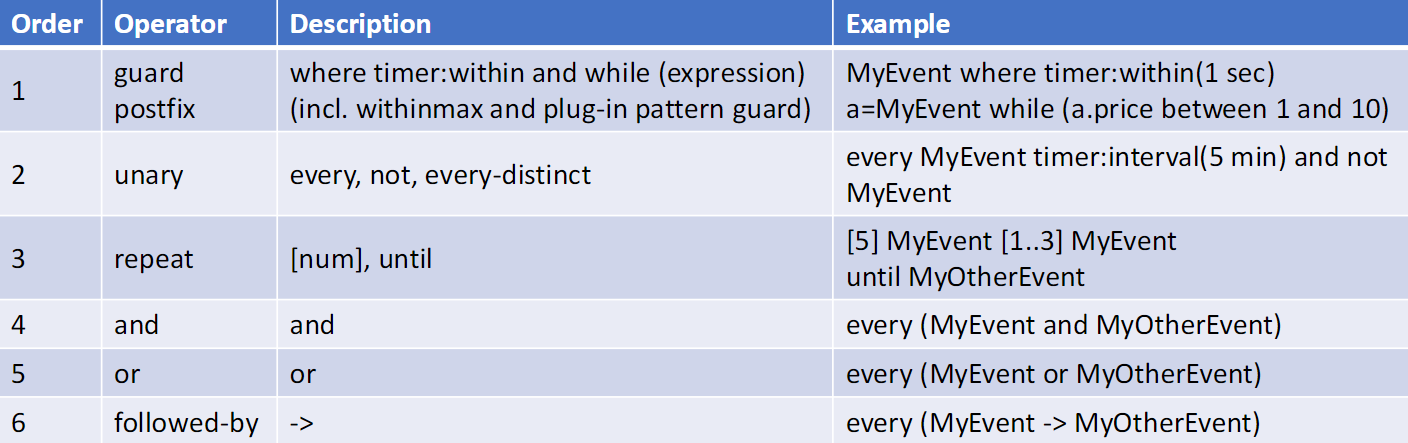
\includegraphics[width=0.95\textwidth]{figures/image_op_precedence_EPL_CEP.png}
    \caption{Operators precedence}
    \label{fig:operators_precedence}
\end{figure}

\subsection{Composing queries}

Typically, queries in EPL are placed in a network. In this way, we can make 
queries interact with each other, and we can define the order in which they are
executed. This allows us to define complex queries by composing simpler ones.\\

\begin{figure}[H]
    \centering
    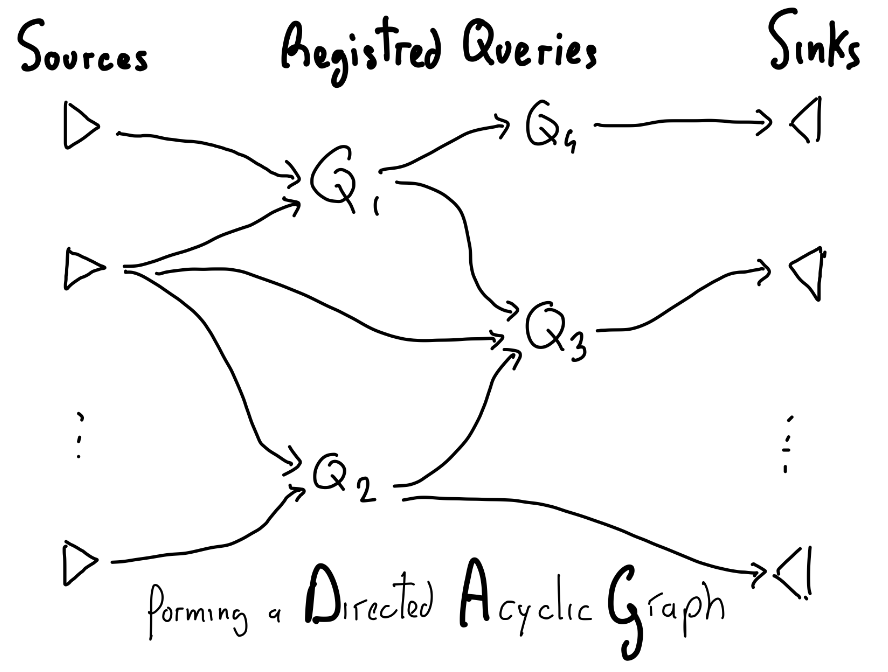
\includegraphics[width=0.5\textwidth]{figures/image_composite_queries.png}
    \caption{Query network}
    \label{fig:query_network}
\end{figure}

We use the \texttt{INSERT INTO} statement to insert the results of a query
into a stream. In this way, we can use the results of a query as input for
another query. Let's see an example of this:\\

\begin{lstlisting}[language=SQL]
@Name('Query_15')
insert into FireEvent
select a.sensor, a.smoke, b.temperature
from pattern [
    every (
        a=SmokeSensorEvent(smoke=true) 
        ->
        b=TemperatureSensorEvent(temperature > 50, sensor = a.sensor)
        where timer:within(2 minutes)
    )
];
\end{lstlisting}

In this query, we are searching for a smoke event followed by a temperature $> 50$
event, within 2 minutes. If the pattern is matched, the results are inserted into
the \texttt{FireEvent} stream. Then, we can use this query:\\

\begin{lstlisting}[language=SQL]
@Name('Query_16')
select count(*)
from FireEvent.win:time(10 minutes);
\end{lstlisting}

In this query, we are counting the number of fire events detected in the last
10 minutes. This way, we can use the results of the first query as input for the
second query.


\section{Joins in EPL}

In SQL, joins are performed on tables, whic are static data structures. The semantics
of SQL joins are based on relational data model and queries that work with complete 
data sets. These joins do not consider the time dimension of the data.\\

In EPL, joins are performed on event streams, which are dynamic data structures. The
semantics of EPL joins are based on event streams and queries that work with continuous
data. These joins intrinsically consider the time dimension of the data.\\

Generally, joins are classified in 3 main types:

\begin{itemize}
    \item Inner join: it returns only the rows that have matching values in both tables.
    \item Left/ight join: it returns all the rows from the left/right table, and the matched rows from the other table.
    \item Full join: it returns all the rows when there is a match in one of the tables.
\end{itemize}

Note that this is true for SQL and EPL. Also based on the structure on which the join is 
performed, in EPL we can distinguish between 3 types of joins:

\begin{itemize}
    \item Stream to stream joins
    \item Table to table joins
    \item Stream to table joins (and viceversa)
\end{itemize}

Note that complex event pattern matching (CEP), seen in the previous section, is a form of join, 
where the join condition is based on the temporal order of the events.

\subsection{Stream to stream joins}

Stream to stream joins are used to join 2 event streams. In each stream, we specify
a window to define the time frame in which the join is performed. For example,
if we use a window of 5 seconds, we will only consider the events that arrive in
the last 5 seconds. Its syntax is as follows:\\

\begin{lstlisting}[language=SQL]
select *
from View#time(9 sec) as v
    inner join
    Click#time(9 sec) as c
    on v.id = c.id;
\end{lstlisting}

In this query, we are joining the \texttt{View} and \texttt{Click} streams on the
\texttt{id} field. We are using a window of 9 seconds for each stream. This way,
we are only considering the events that arrive in the last 9 seconds.\\

Consider that the queries are only executed when an event arrives in the stream, 
and only returns the new results that match the join condition. The following figure 
describes the process of a stream to stream (inner) join:

\begin{figure}[H]
    \centering
    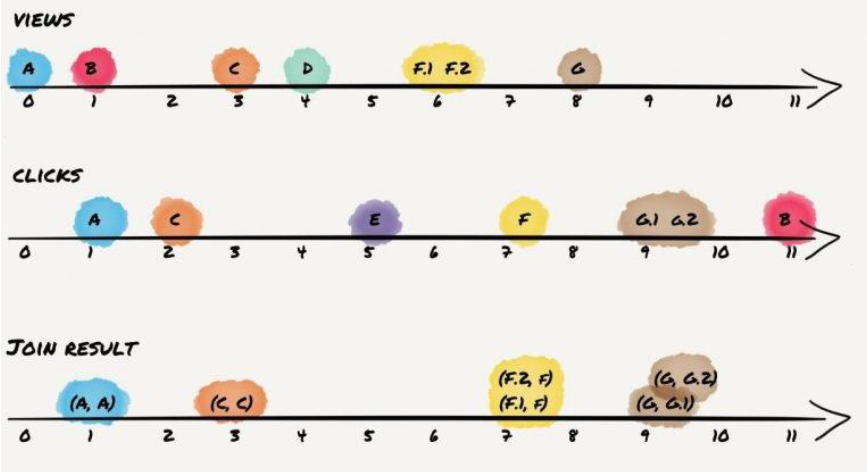
\includegraphics[width=0.7\textwidth]{figures/image_stream_stream_join.png}
    \caption{Stream to stream join}
    \label{fig:stream_stream_join}
\end{figure}

Note that we can also perform left/right outer joins and full outer joins. The
syntax is similar to the inner join, but we use the \texttt{left outer join},
\texttt{right outer join}, and \texttt{full outer join} statements, respectively.\\

Joins among streams have profoundly different semantics, because they are designed to
run on real-time data streams, essentially unbounded record sequences. Events are joined
only if they arrive within a specific time window. This temporal aspect is central and 
instrinsic to the join semantics of streams. The concept of time is crucial, as Joins
depend on the time synchronization of the events in the streams, which instroduces a 
significant difference with respect to traditional SQL joins.

\subsection{Table to table joins}

EPL offers 3 ways to build a table from an event stream:

\begin{itemize}
    \item \texttt{KEEP ALL}: this window is one that retains all arriving events. However,
    take should be taken to remove events from the window, in a timely manner.
    \item \texttt{UNIQUE}: this window is one that retains only the most recent event for
    each unique key. 
    \item \texttt{CREATE TABLE} with \texttt{INSERT INTO}: this window is one that retains
    all arriving events, but it is not a window in the sense of a time window.
\end{itemize}

We will mainly use the \texttt{UNIQUE} window to build tables from event streams. This
window is one that retains only the most recent event for each unique key. Its syntax is
as follows:\\

\begin{lstlisting}[language=SQL]
select *
from View#unique(id) as v
    inner join
    Click#unique(id) as c
    on v.id = c.id;
\end{lstlisting}

In this query, we are joining the \texttt{View} and \texttt{Click} streams on the
\texttt{id} field. We are using the \texttt{unique} window to build tables from the
event streams. This way, we are only considering the most recent event for each unique
key, in this case, the \texttt{id} field.\\

Note that we are not actually joining tables, but event streams. The tables are built
from the event streams, and the join is performed on these tables. So we call them 
"tables" as they seem to inherit the unique key constraint from the SQL tables. The
following figure describes the process of a table to table (inner) join:

\begin{figure}[H]
    \centering
    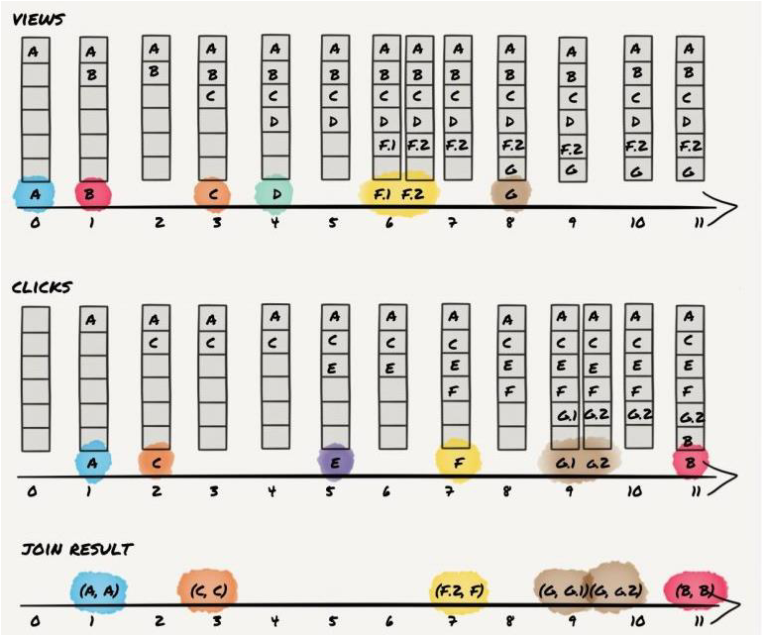
\includegraphics[width=0.6\textwidth]{figures/image_table_table_join.png}
    \caption{Table to table join}
    \label{fig:table_table_join}
\end{figure}

Note that the events persist over time, only being replaced by newer events with the same
key. This is a key difference with respect to stream to stream joins, where the events are
only considered within a specific time window.\\

We can also perform left/right outer joins and full outer joins. The syntax is similar to
the inner join, but we use the \texttt{left outer join}, \texttt{right outer join}, and
\texttt{full outer join} statements, respectively.

\subsection{Stream to table joins}

These type of joins introduce a new keyword: \texttt{UNIDIRECTIONAL}. This keyword is used in
the \texttt{JOIN} clause to identify streams that provide the events to execute the join. If
the keyword is present for a stream, all other streams in the \texttt{FROM} clause become
passive streams. That means that when a new event arrives or leaves a data window of a passive
stream, the join does not generate new results.\\

Therefore, the \texttt{UNIDIRECTIONAL} keyword makes the stream-to-table join asymmetric: only
the input from the stream with the \texttt{UNIDIRECTIONAL} keyword will trigger the join. And 
because the join is not-windowed, this stream is stateless; thus join lookups from the table 
to the stream are not possible.\\

The syntax for a stream to table join is as follows:\\

\begin{lstlisting}[language=SQL]
select *
from View as v
    unidirectional inner join
    Click#unique(id) as c
    on v.id = c.id;
\end{lstlisting}

In this query, we are joining the \texttt{View} stream with the \texttt{Click} table on the
\texttt{id} field. We are using the \texttt{unique} window to build the table from the
\texttt{Click} stream. This way, we are only considering the most recent event for each
unique key, in this case, the \texttt{id} field. In this case, a new click event won't
trigger the join, but a new view event will, and because the stream is stateless, join
lookups from the Click table to the View stream are not possible.\\

The following figure describes the process of a stream to table (inner) join:

\begin{figure}[H]
    \centering
    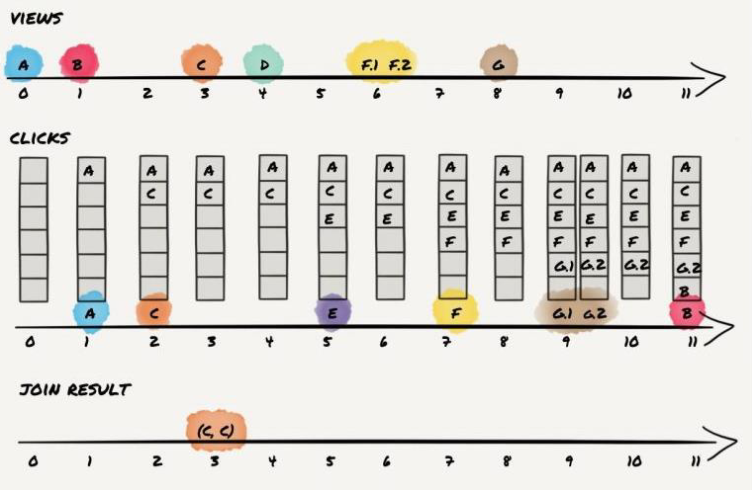
\includegraphics[width=0.62\textwidth]{figures/image_stream_table_join.png}
    \caption{Stream to table join}
    \label{fig:stream_table_join}
\end{figure}

We can also perform left/right outer joins and full outer joins. The syntax is similar to
the inner join, but we use the \texttt{left outer join}, \texttt{right outer join}, and
\texttt{full outer join} statements, respectively.

\section{Contexts in EPL}

In EPL, we can also define contexts. A context enables more flexible and stateful processing
in scenarios requiring grouping or conditions that go beyond simple event windows. In fact, 
contexts define a new type of window (different than tumbling and hopping windows), which we 
will name a session window.\\

Why use contexts? Here is a list of advantages:

\begin{itemize}
    \item[$\rightarrow$] Better control: context gives fine-grained control over how events are processed.

    \item[$\rightarrow$] Stateful processing: handles cases where the state is important, e.g., sessions or
    transactions.

    \item[$\rightarrow$] Efficient partitioning: it helps reduce complexity in event, partitioning by user, 
    session, or custom logic.
\end{itemize}

We have three main types of contexts:

\begin{itemize}
    \item Context by key: partitions events based on a key, e.g., \texttt{userId}.

    \item Context by start/end conditions: defined by specific events or triggers.

    \item Context by time: defines temporal windows (generalizes logical windows, e.g., it allows
    to declare session windows).
\end{itemize}

\subsection{Context by key}

Context by key is used to partition events based on a key. It is useful when we want to group
events by a specific attribute, e.g., \texttt{userId}. Its syntax is as follows:\\

\begin{lstlisting}[language=SQL]
create context UserSessionContext
partition by userId from UserActionEvent;
\end{lstlisting}

In this context, we are partitioning events by the \texttt{userId} attribute from the
\texttt{UserActionEvent} stream. This way, we are grouping events by the \texttt{userId}
attribute. Note that this process is highly parallelizable, as each partition can be processed
independently.

\subsection{Context by start/end conditions}

Context by start/end conditions is defined by specific events or triggers. It is useful when we
want to group events based on specific conditions, e.g., when a session starts or ends. Its syntax
is as follows:\\

\begin{lstlisting}[language=SQL]
create context OrderContext
initiated by OrderEvent(orderStatus = 'NEW')
terminated by OrderEvent(orderStatus = 'COMPLETED');
\end{lstlisting}

In this context, we are defining a session window that starts when an \texttt{OrderEvent} with
\texttt{orderStatus = 'NEW'} arrives and ends when an \texttt{OrderEvent} with \texttt{orderStatus
= 'COMPLETED'} arrives. This way, we are grouping events based on the start and end conditions.\\

Note that we could use this context along with the context by key to partition events based on a key
and start/end conditions. Look at the following example:\\

\begin{lstlisting}[language=SQL]
create context OrderContext;
partition by userId from UserActionEvent;
initiated by UserActionEvent(action = 'start_order');
terminated by UserActionEvent(action = 'complete_order');
\end{lstlisting}

\subsection{Context by time}

Context by time allows us to track actions within fixed periods of time. They are triggered by some
condition and last for a specific time. Its syntax is as follows:\\

\begin{lstlisting}[language=SQL]
create context TimeBatchContext
partition by userId from UserActionEvent;
initiated by UserActionEvent(action = 'start_order');
terminated after 10 minutes;
\end{lstlisting}

In this context, we are defining a session window that starts when an \texttt{UserActionEvent} with
\texttt{action = 'start\_order'} arrives and ends after 10 minutes. This way, we are grouping events
based on the time window. Note that we are also partitioning events by the \texttt{userId} attribute.

\subsection{Comparison: Windows vs. Contexts}

Windows and contexts are both used to group events, but they have different semantics. Let us look
at the following figure that shows the main differences between windows and contexts:

\begin{figure}[H]
    \centering
    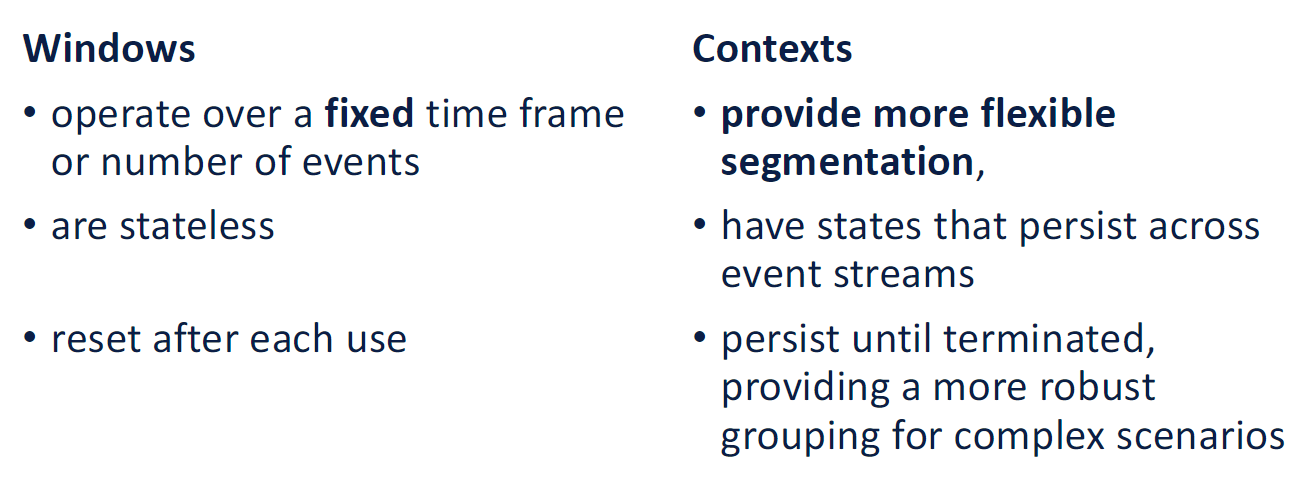
\includegraphics[width=0.8\textwidth]{figures/image_windows_vs_context.png}
    \caption{Windows vs. Contexts}
    \label{fig:windows_vs_contexts}
\end{figure}
